\documentclass[12pt]{article}
\usepackage[utf8]{inputenc}
\usepackage{amsmath}
\usepackage{graphicx}
\usepackage{float}
\usepackage{breqn}
\usepackage[margin=1in]{geometry}
\usepackage{lineno}
\setlength{\parskip}{1em}
\renewcommand{\baselinestretch}{1.5}
\newcommand\dbyd[2]{\frac{\mathrm d{#1}}{\mathrm d{#2}}}
\newcommand\dsided[2]{{\mathrm d{#1}}/{\mathrm d{#2}}}
\newcommand{\R}{\mathcal{R}}
\title{Some plots I made to fix/answer some of the problems in my draft}
\author{Roger Zhang}
\date{July 16th 2018}
\usepackage{color}
\newcommand{\david}[1]{\textcolor{blue}{$\langle${\slshape{\bfseries David:} #1 }$\rangle$}}
\newcommand{\roger}[1]{\textcolor{red}{$\langle${\slshape{\bfseries Roger:} #1 }$\rangle$}}
\usepackage[colorlinks=true,linkcolor=blue]{hyperref}
\newcommand{\pmV}{p_{V}}
\newcommand{\pmI}{p_{I}}
\begin{document}
\maketitle
\clearpage
\section{Region of $(\R_0,p)$ plane where there are damped
  oscillations (fixed $\epsilon$)}

$p$ is the proportion of intentional infection and $\R_0$ is the basic reproduction number.

Here I show several plot with different $\epsilon$ in increasing order. In the following graphs, the shaded area represent the region where the system has damped oscillation.
\subsection{$\epsilon=\frac{7}{18257}$}
\begin{figure}[H]
  \caption{}
  \centering
  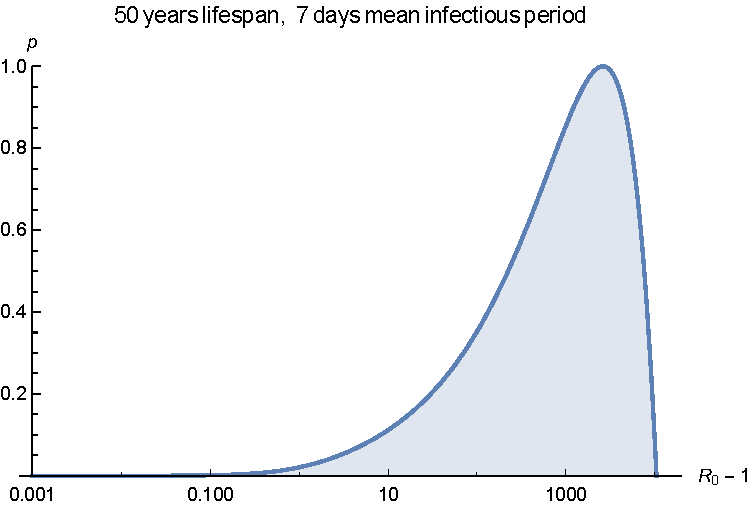
\includegraphics[width=0.9\textwidth]{Figures/50_7.pdf}
\end{figure}

\subsection{$\epsilon=\frac{11}{9136}$}
\begin{figure}[H]
  \caption{}
  \centering
  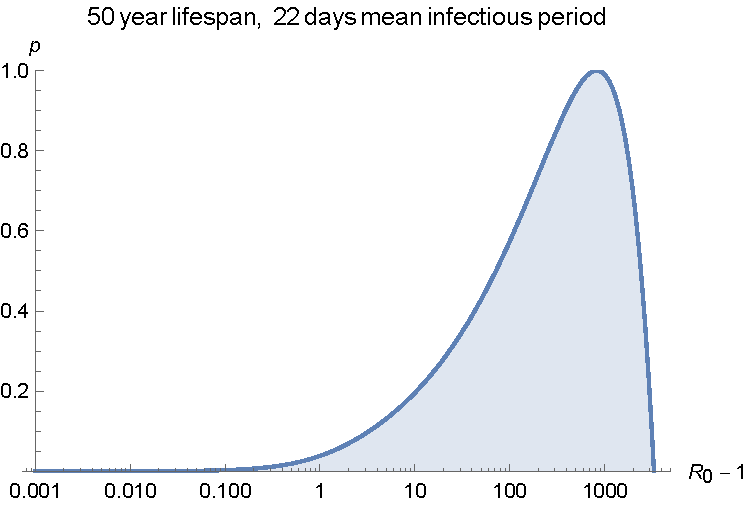
\includegraphics[width=0.9\textwidth]{Figures/50_22.pdf}
\end{figure}

\subsection{$\epsilon=\frac{1}{51}$}
\begin{figure}[H]
  \caption{}
  \centering
  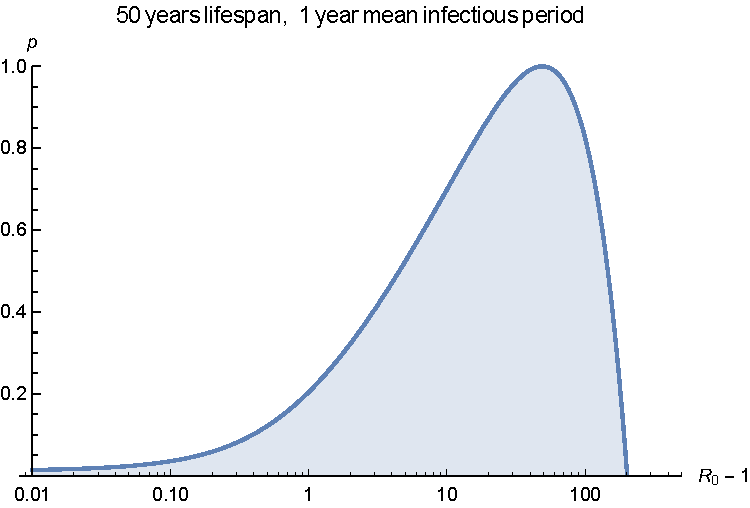
\includegraphics[width=0.9\textwidth]{Figures/50_365.pdf}
\end{figure}

\subsection{$\epsilon=\frac{1}{10000}$}
\begin{figure}[H]
  \caption{}
  \centering
  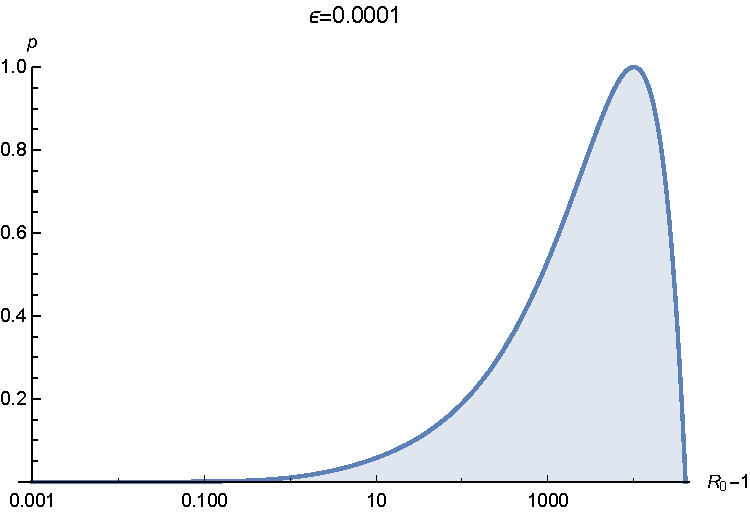
\includegraphics[width=0.9\textwidth]{Figures/epsilon_0_0001.pdf}
\end{figure}

\subsection{$\epsilon=\frac{1}{1000}$}
\begin{figure}[H]
  \caption{}
  \centering
  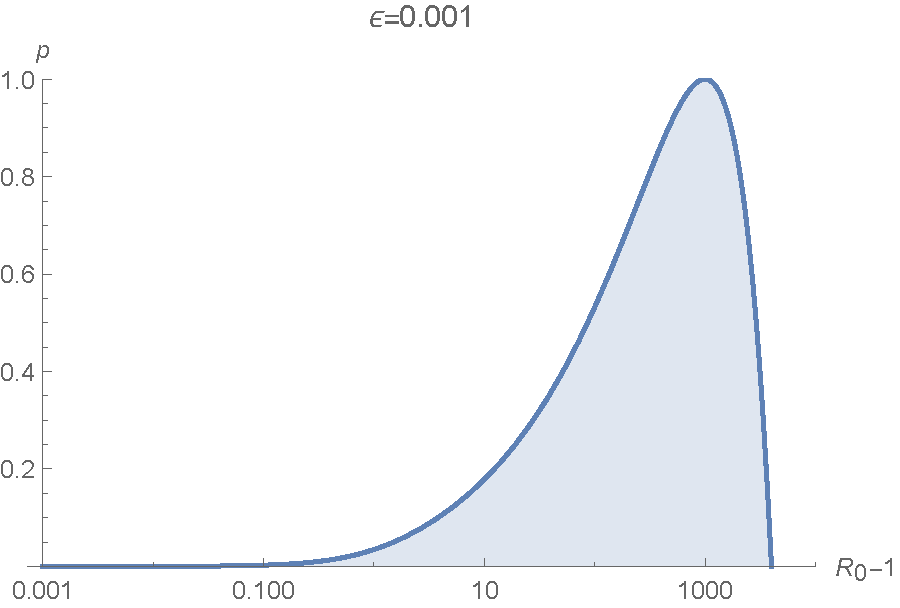
\includegraphics[width=0.9\textwidth]{Figures/epsilon_0_001.pdf}
\end{figure}

\subsection{$\epsilon=\frac{1}{100}$}
\begin{figure}[H]
  \caption{}
  \centering
  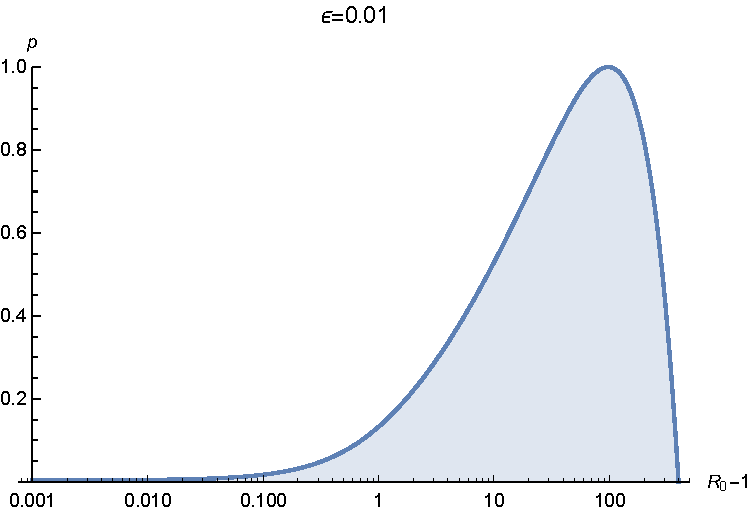
\includegraphics[width=0.9\textwidth]{Figures/epsilon_0_01.pdf}
\end{figure}

\subsection{$\epsilon=\frac{1}{10}$}
\begin{figure}[H]
  \caption{}
  \centering
  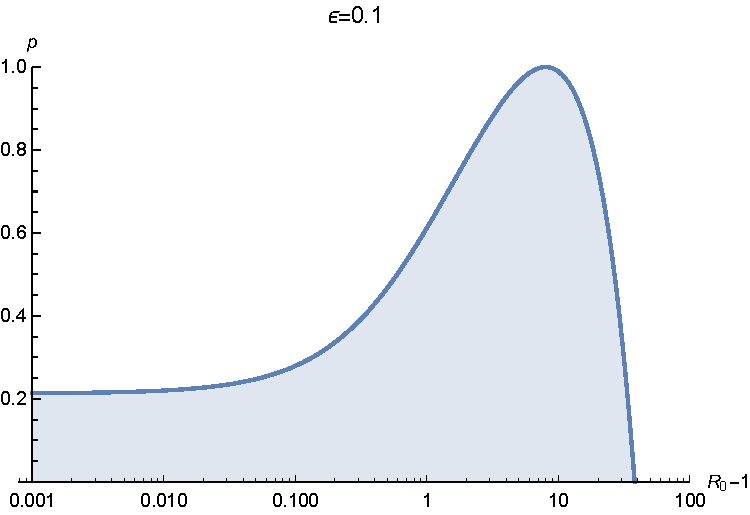
\includegraphics[width=0.9\textwidth]{Figures/epsilon_0_1.pdf}
\end{figure}

\subsection{$\epsilon=0.5$}
\begin{figure}[H]
  \caption{}
  \centering
  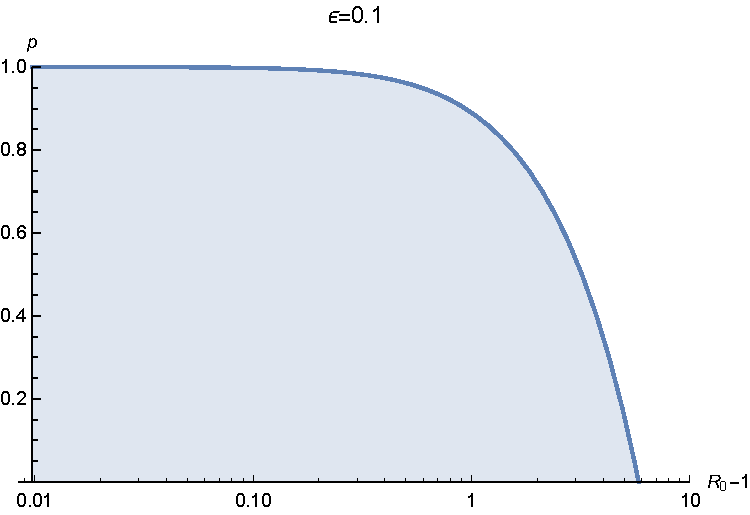
\includegraphics[width=0.9\textwidth]{Figures/epsilon_0_5.pdf}
\end{figure}
\clearpage


\section{Region of $(\R_0,\epsilon)$ plane where there are damped
  oscillations (fixed $p$)}

Again, I made plots with different $p$ in increasing order, the shade area between the blue curve and the orange curve represent the region where the system has damped oscillation.
\subsection{$p=0$}
\begin{figure}[H]
  \caption{}
  \centering
  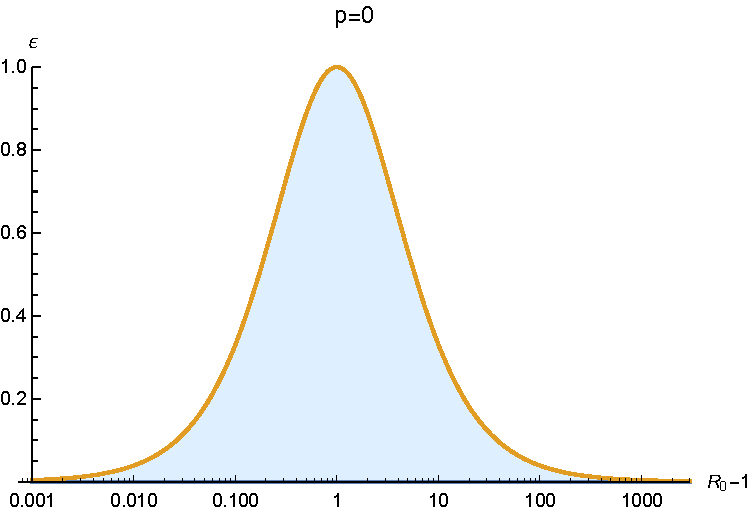
\includegraphics[width=1\textwidth]{Figures/p_0.pdf}
\end{figure}

\subsection{$p=0.2$}
\begin{figure}[H]
  \caption{}
  \centering
  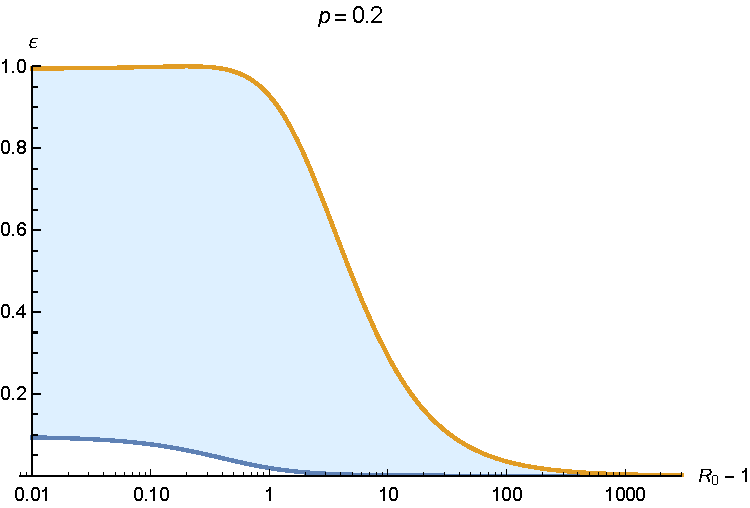
\includegraphics[width=1\textwidth]{Figures/p_0_2.pdf}
\end{figure}

\subsection{$p=0.5$}
\begin{figure}[H]
  \caption{}
  \centering
  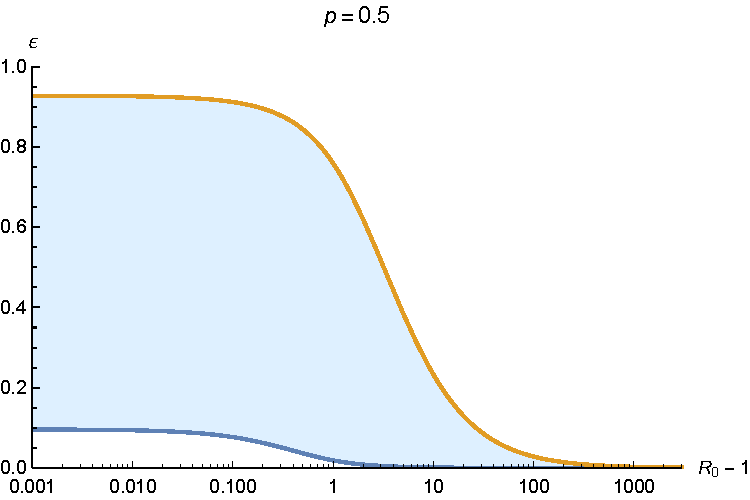
\includegraphics[width=1\textwidth]{Figures/p_0_5.pdf}
\end{figure}

\subsection{$p=0.8$}
\begin{figure}[H]
  \caption{}
  \centering
  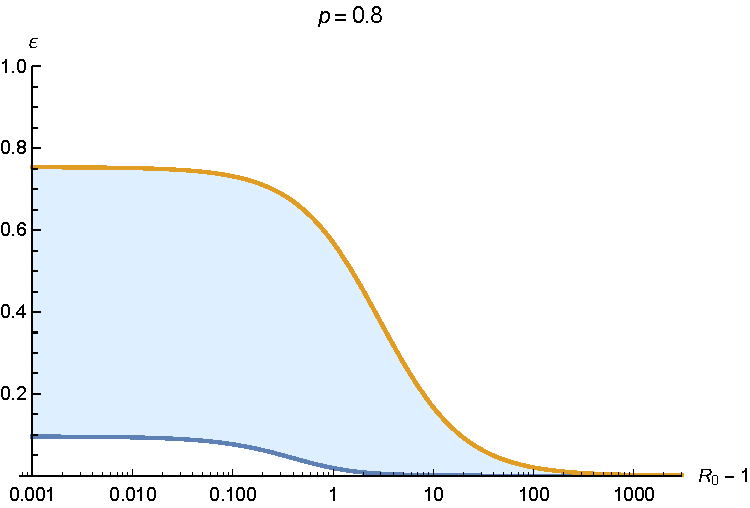
\includegraphics[width=1\textwidth]{Figures/p_0_8.pdf}
\end{figure}
\clearpage
\section{Correct formulation for smallpox and variolation}

Variolation of smallpox is a method of apply live smallpox virus to healthy individuals intentionally, via skin. Here we assume that variolation is done by using the same strain of virus, therefore, individuals infected by variolated cases are also considered to be naturally infected(Secondary cases caused by variolated cases are naturally infected). Skin transmission is usually slower than transmission by air, as a result, we also assume that the transmission rate for variolated cases are slower than naturally infected cases.

The correct formulation based on these assumptions is shown in the following.

\begin{subequations}\label{eq:base_ODE}
\begin{align}
\dbyd{S}{\tau}&=\epsilon(1-p)-\R_{0,V} SV-\R_{0,I} SI-\epsilon S\,, \label{eq:S_by_tau}\\
\dbyd{V}{\tau}&=\epsilon p-V\,, \label{eq:V_by_tau}\\
\dbyd{I}{\tau}&=\R_{0,V} SV+\R_{0,I} SI-I\,, \label{eq:I_by_tau}\\
\dbyd{M}{\tau}&=\pmV(1-\epsilon) V+\pmI(1-\epsilon) I\,,\\
\dbyd{R}{\tau}&=(1-\pmV)(1-\epsilon) V+(1-\pmI)(1-\epsilon) I-\epsilon R\,.
\end{align}
\end{subequations}
Here, $R_{0,I}$ and $R_{0,I}$ are basic reproduction number for naturally infected and variolated cases.


\subsection{Equilibrium}

By solving the system, we obtain one equilibrium,
\begin{subequations}
\begin{align}
\hat{S}&=\frac{1+\R_{0,V}p+\R_{0,I}-\R_{0,I}p-\sqrt{4(p-1)\R_{0,I}+(1+\R_{0,V}p+\R_{0,I}-\R_{0,I}p)^2}}{2\R_{0,I}}\,,\\ \label{Shat}
\hat{V}&=\epsilon p\,,\\
\hat{I}&=\frac{\epsilon}{2}(1-p-\frac{1}{\R_{0,I}}+\frac{\sqrt{4(p-1)\R_{0,I}+(1+\R_{0,V}p+\R_{0,I}-\R_{0,I}p)^2}}{\R_{0,I}})\,.
\end{align}
\end{subequations}

Notice, $\hat{I}$ reduces to 0 for $p=1$, and reduces to $\epsilon(1-\frac{1}{\R_{0,I}})$ for $p=0$.

Since $\hat{V}$ and $\hat{I}$ cannot both equal to 0 for any choice of $p$ between 0 and 1, this equilibrium is not a disease free equilibrium, but an endemic equilibrium(EE).
\subsection{Stability at EE}
Jacobian of this system is:
\begin{equation}
\mathcal{J} =
\begin{bmatrix}
    \ -\R_0 (V+I)-\epsilon       & -\R_0 S     &-\R_0 S\\
    \ 0       & -1    &0\\
    \ \R_0 (V+I)       &\R_0 S     &\R_0 S-1\\
\end{bmatrix}\,.
\end{equation}
Eigenvalues of Jacobian are:
\begin{subequations}
\begin{align}
\lambda_1&=-1\,,\\ \label{lam2}
\lambda_2&=\frac{-1-\R_{0,I}(I-S)-\R_{0,V}V-\epsilon-\sqrt{(1+\R_{0,I}(I-S)+\R_{0,V}V+\epsilon)^2-4(\R_{0,I}(I-S\epsilon)+\R_{0,V}V+\epsilon)}}{2}\,,\\ \label{lam3}
\lambda_3&=\frac{-1-\R_{0,I}(I-S)-\R_{0,V}V-\epsilon+\sqrt{(1+\R_{0,I}(I-S)+\R_{0,V}V+\epsilon)^2-4(\R_{0,I}(I-S\epsilon)+\R_{0,V}V+\epsilon)}}{2}\,.
\end{align}
\end{subequations}

By using \autoref{Shat}, \autoref{lam2} and \autoref{lam3}, we can prove that,
\begin{equation}
\frac{-1-\R_{0,I}(I-S)-\R_{0,V}V-\epsilon}{2}<0
\end{equation}

If the quantity under the square root is positive, then $\Re(\lambda_2)<\Re(\lambda_3)<0$.

Otherwise, if the quantity under the square root is negative,
\begin{equation}
\Re(\lambda_2)=\Re(\lambda_3)=\frac{-1-\R_{0,I}(I-S)-\R_{0,V}V-\epsilon}{2}<0
\end{equation}
Therefore, the equilibrium at EE is locally stable.
\clearpage
\section{Effect of variolation on mortality}
\subsection{Mortality at EE}
As shown in \autoref{IatEE}, $\hat{I}$ decreases as $p$ increases. Therefore, $\dbyd{M}{\tau}$ decreases as $p$ increases. Meaning, a larger proportion of variolation will lead to fewer death in the long run.
\begin{figure}[H]
  \caption{$\hat{I}$ as a function of $p$}
  \centering\label{IatEE}
  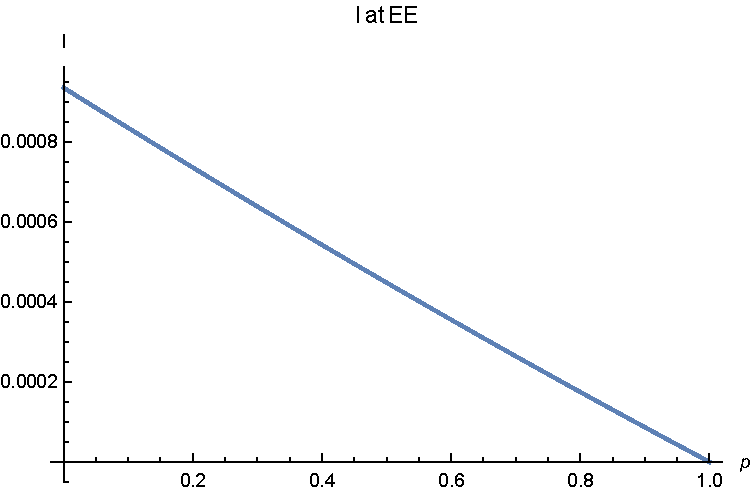
\includegraphics[width=1\textwidth]{Figures/I_at_EE.pdf}
\end{figure}

\subsection{Total mortality}
We run numerical simulations with the following initial condition,
\begin{subequations}
\begin{align}
\hat{S}&=\frac{1}{\R_{0,I}}\,,\\
\hat{V}&=\epsilon p\,,\\
\hat{I}&=\epsilon(1-\frac{1}{\R_{0,I}})
\end{align}
\end{subequations}
For smallpox, parameter values in \autoref{tab:params} are used, 
\begin{table}[H]
\begin{center}
\caption{Model parameters and smallpox values.}
\label{tab:params}
\smallskip
\begin{tabular}{c|c|r}
{\bfseries Symbol} & {\bfseries Meaning} & {\bfseries Value} \\\hline
$\mu$ & Natural \emph{per capita} death rate & $\frac{1}{50*365}$ per day \\
$\gamma$ & Recovery rate & $\frac{1}{22}$ per day \\
$\R_{0,I}$ & Basic reproductive number(Naturally) & 4.5\\
$\R_{0,V}$ & Basic reproductive number(Variolated) & 2.5
\end{tabular}
\end{center}
\end{table}

We assume that, transmission rate for variolated cases is slower than naturally infected cases, therefore $\R_{0,V}<\R_{0,I}$.

\begin{figure}[H]
  \centering\label{IatEE}
  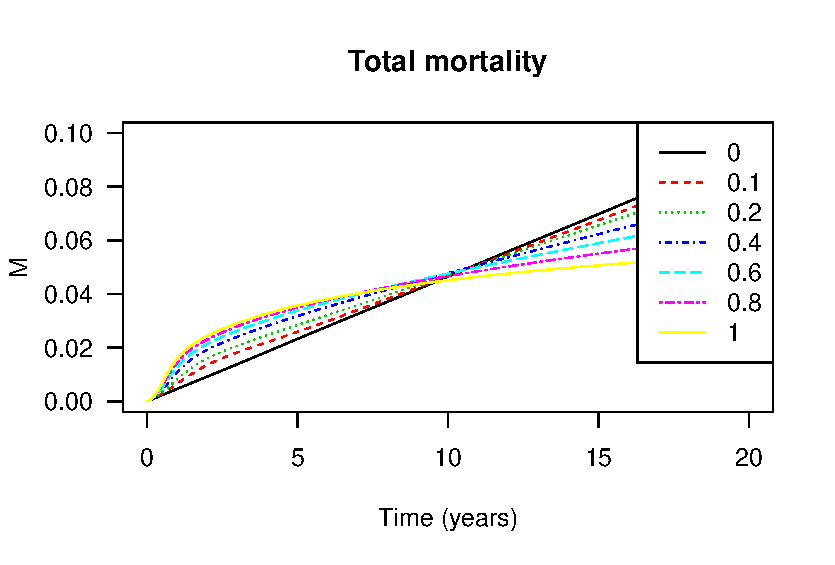
\includegraphics[width=1\textwidth]                 {Figures/Total_Mortality.pdf}
  \caption{Total Mortality as a function of time}
\end{figure}

We are also interested in the time it takes for variolation ($p>0$) to become
advantagous compared with not variolating anybody ($p=0$).

\begin{figure}[H]
  \centering\label{Variolation_advantage}
  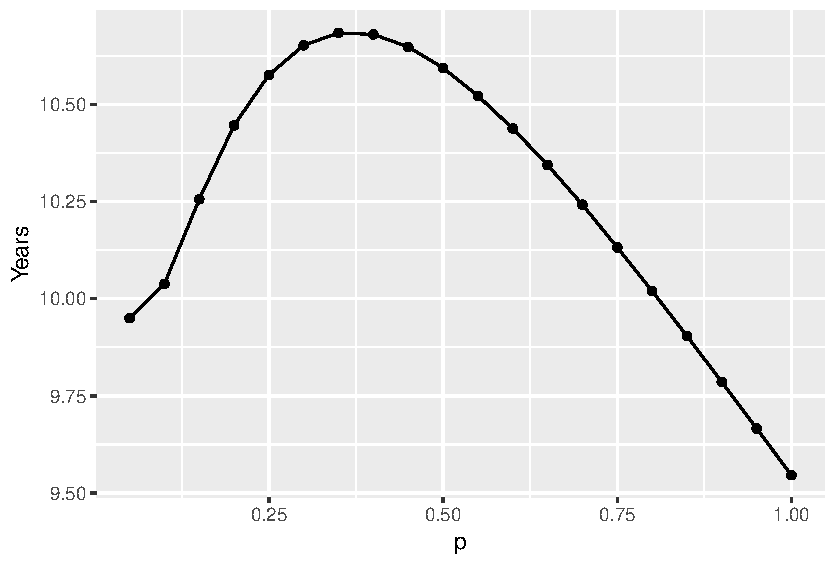
\includegraphics[width=1\textwidth]                 {Figures/Variolation_advantage_time.pdf}
  \caption{Time required for variolation to become advantagous after
    it is introduced into a population at the SIR endemic
    equilibrium.  Note that the vertical scale is quite narrow in this
  graph.}\label{Variolation_time_advantage}
\end{figure}

From \autoref{Variolation_time_advantage}, we can see that $p=1$ is not only proven to be more beneficial in the long run, but also takes less time to gain advantage over non-variolation, by having less total mortality.

\end{document}
